%%%%%%%%%%%%%%%%%%%%%%%%%%%%%%%%%%%%%%%%%
% Diaz Essay
% LaTeX Template
% Version 2.0 (13/1/19)
%
% This template originates from:
% http://www.LaTeXTemplates.com
%
% Authors:
% Vel (vel@LaTeXTemplates.com)
% Nicolas Diaz (nsdiaz@uc.cl)
%
% License:
% CC BY-NC-SA 3.0 (http://creativecommons.org/licenses/by-nc-sa/3.0/)
%
%%%%%%%%%%%%%%%%%%%%%%%%%%%%%%%%%%%%%%%%%

%----------------------------------------------------------------------------------------
%	PACKAGES AND OTHER DOCUMENT CONFIGURATIONS
%----------------------------------------------------------------------------------------

\documentclass[11pt]{diazessay} % Font size (can be 10pt, 11pt or 12pt)
\usepackage[export]{adjustbox}
\usepackage{subcaption}
%----------------------------------------------------------------------------------------
%	TITLE SECTION
%----------------------------------------------------------------------------------------

\title{\textbf{Report} \\ {\Large\itshape Doggos emotions recognition and classification}} % Title and subtitle

\author{\textbf{Artificial Inteligence} \\ \textit{Anna Przybycien, Agnieszka Szlendak}} % Author and institution

\date{\today} % Date, use \date{} for no date

%----------------------------------------------------------------------------------------

\begin{document}

\maketitle % Print the title section

%----------------------------------------------------------------------------------------
%	ABSTRACT AND KEYWORDS
%----------------------------------------------------------------------------------------

%\renewcommand{\abstractname}{Summary} % Uncomment to change the name of the abstract to something else

\begin{abstract}

\end{abstract}

%\hspace*{3.6mm}\textit{Keywords:} emotion recognition, CNN, doggos, wisdom, %knowledge, hudge mess, majnas % Keywords

\vspace{10pt} % Vertical whitespace between the abstract and first section

%----------------------------------------------------------------------------------------
%	ESSAY BODY
%----------------------------------------------------------------------------------------

\section*{Data preparation}
In order to create a model for classification we needed proper dataset with dogs images. Unfortunatelly, for now, there is no proper dataset published suited for dogs emotion recognition. We were faced with the challenge of creating the dataset by ourselfes. The task consisted of four major parts:
\begin{enumerate}
	\item Finding the data source. \\
	As downloading images manually from google graphics would be too much of a hussle, we decided to use a tool 4K Stogram, which enabled us to download pictures based on tags from Instagram directly on our discs.
	\\
	\item Defining number and characteristics of classes. \\ 
	Because of the time and resource access constraint, we had to limit the number of classes to four. We also vaguely assumed what are the characteristics of each class:
	\begin{itemize}
		\item \textbf{happy dogs} - dogs with the smile, mainly with open muzzle and tongue out
		\item \textbf{angry dogs} - dogs that looks scary, with their teeth showing
		\item \textbf{sleepy dogs} - dogs that are taking a nap, or are about to, with closed or squinted eyes,
		\item \textbf{good dogs} - dogs that looks polite, with neutral muzzle \\
	\end{itemize} 
	\item Determining classes numerousity \& dataset creation. \\ 
	First, we assume that minimum number of images for each class should be 500. We began dataset preparation with the phrase 'the bigger the better' in mind, but we were able only to reach our assumed baseline of 500 per class.
	So, from that point forward, we had dataset of 2000 classified images.\\
	\item Seperating into train, validation and test sets.\\ 
	Lastly, as our dataset was small, we proceed to separate it using 60/20/20 proportion:
	\begin{itemize}
		\item 60\% - 1200 (300 per class) images in training set
		\item 20\% - 400 (100 per class) images in validation set
		\item 20\% - 400 (100 per class) images in test set
	\end{itemize}
	
\end{enumerate}
\section*{AI implementation}
\begin{itemize}

	\item pure CNN \\
We started with the simplest neural network we could think of, one consisting of four layers - every one used relu as its activation function - and one with softmax at the end. \\We went for 30 epochs and achieved 30\% accuracy on validation data. Despite tremendous overitting we were off to a good start.  
	\item CNN with data augmentation \\
Overfitting was due to small size of our dataset, but it turned out that keras has perfect solution for it - easy to implement data augumentation - process that from one sample creates more by subjecting ir to various transformations. \\
This time we decided on 100 epochs, so after some time (even using GPU) we got 56\% accuracy with overfitting at smaller scale.   
	\item CNN with convolutional base taken from 'imagenet' \\
	To counter overfitting resulting from using small dataset, we decided to use transfer learning and introduce convolutional base, pre-trained on famous imagenet dataset. Imagenet includes pictures of all sorts of animals, including various breeds of dogs, so we cocluded it would be suitable for our needs. It performed much better than pure version, with ~60\% accuracy and similar to the version with data augmentation.
	\begin{figure}[h]
 
	\begin{subfigure}{0.5\textwidth}
    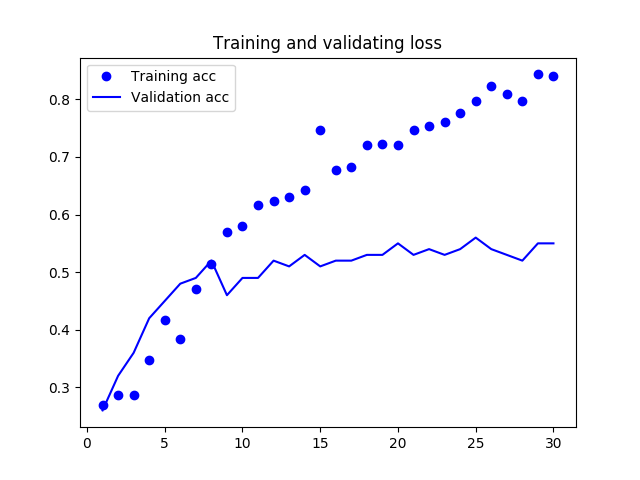
\includegraphics[scale=0.4, left]{cnn-imgenet-acc.png}
    \caption{Accuracy function}
    \label{fig:subim1}
    \end{subfigure}
    \begin{subfigure}{0.5\textwidth}
	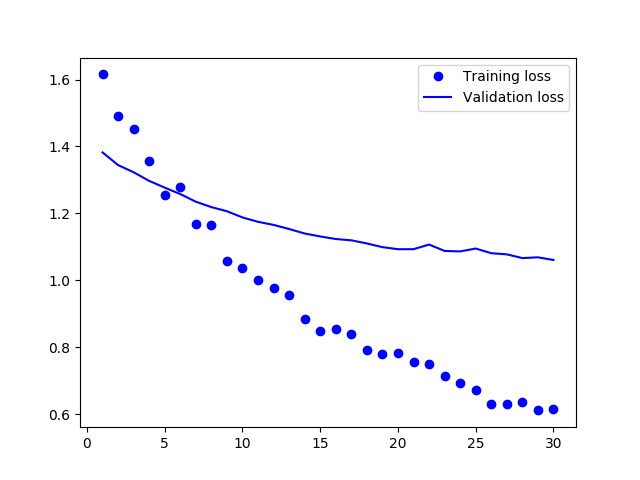
\includegraphics[scale=0.4, right]{cnn-imgenet-loss.png}
    \caption{Loss function}
    \label{fig:subim2}
    \end{subfigure}
 
    \caption{Accuracy and loss functions for CNN with 'imagenet'}
    \label{fig:image2}
    \end{figure}
	
	
    
	\item CNN with convolutional base taken from 'imagenet' with data augmentation and early stopping\\
	
\end{itemize}
%------------------------------------------------


\section*{Final remarks}

%\begin{center}%{l}{1\textwidth} % Inline image example, use an 'r' column type to position the figure on the right
%	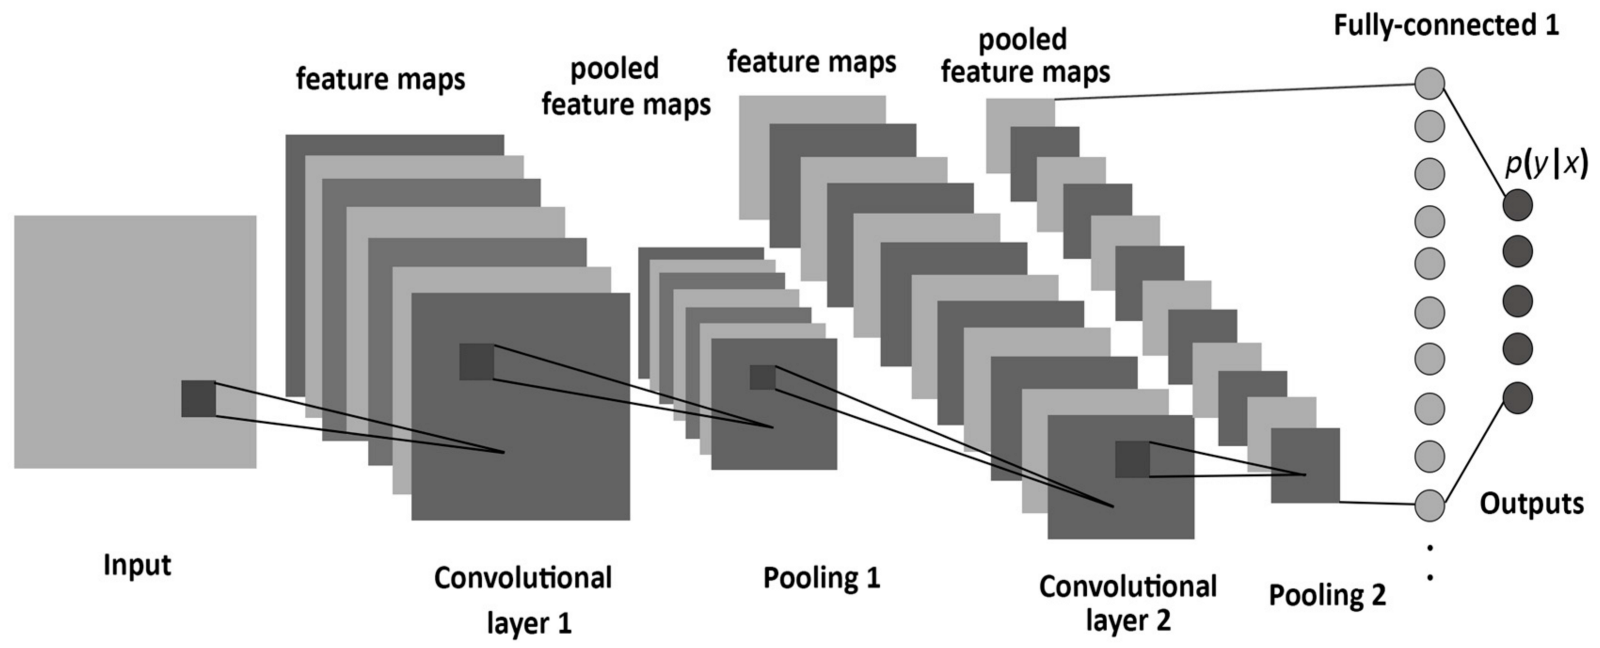
\includegraphics[scale=0.2]{cnn.png}
%	\caption{An example fish.}
%\end{center}


%------------------------------------------------

%----------------------------------------------------------------------------------------
%	BIBLIOGRAPHY
%----------------------------------------------------------------------------------------
\section*{Sources}
\begin{itemize}
\item
  \textit{Deep Learining with Python}, Fracouis Chollet.
\end{itemize}

%----------------------------------------------------------------------------------------

\end{document}
